\documentclass[12pt]{article}

\usepackage{graphicx}
\usepackage[margin=3cm]{geometry}
\usepackage{pdfpages}
\usepackage{minted}

\author{Pablo Vargas Bermúdez}

\begin{document}
\pagestyle{empty}

\includepdf[pages=-]{Portada}

\section*{Planteamiento}
Crea una interfaz gráfica donde muestres el uso del GridbagLayout y
donde coloques una serie de botones distribuidos de la siguiente
manera:

\begin{center}
  \includegraphics[width=.5\textwidth]{figures/muestra.jpg}
\end{center}

Envía un archivo PDF que contenga una hoja de presentación, la
descripción de la tarea, el código fuente de la solución y anexa
también las pantallas necesarias donde muestres el correcto
funcionamiento del programa funcionamiento.

\section*{Código}
\subsection*{Gui}
\inputminted{Java}{Gui.java}
\subsection*{Prueba}
\inputminted{Java}{Prueba.java}

\section*{Ejecución}
\begin{figure}[ht]
  \centering
  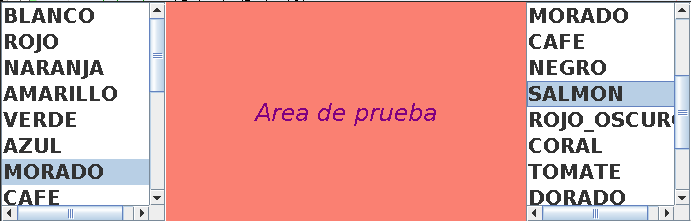
\includegraphics[width=\textwidth]{figures/run1.png}
  \caption{Interfaz}
\end{figure}
\end{document}
